%%%%%%%%%%%%%%%%%%%%%%%%%%%%%%%%%%%%%%%%%
%
% (c) 2022 by Jennifer Laaser
%
% This work is licensed under the Creative Commons Attribution-NonCommercial-ShareAlike 4.0 International License. To view a copy of this license, visit http://creativecommons.org/licenses/by-nc-sa/4.0/ or send a letter to Creative Commons, PO Box 1866, Mountain View, CA 94042, USA.
%
% The current source for these materials is accessible on Github: https://github.com/jlaaser/pogil-polymers
%
%%%%%%%%%%%%%%%%%%%%%%%%%%%%%%%%%%%%%%%%%

\renewcommand{\figpath}{content/polymphys/thermal-transitions/thermal-characterization/figs}
\renewcommand{\labelbase}{thermal-characterization}

\begin{activity}{Measuring $T_g$ and $T_m$}

\begin{instructornotes}
	This activity introduces students to concepts related to measuring the glass transition temperatures and melting temperatures of polymer materials.
	
	After completing this activity, students will be able to:
	\begin{enumerate}
		\item Explain how the modulus of a material should change at its $T_g$ and $T_m$, and use measurements of modulus as a function of temperature to identify these transition temperatures
		\item Explain the heat flow signatures expected for glass transitions and melting transitions in DSC, and use DSC data to identify the temperatures at which these transitions occur
	\end{enumerate}
	
	\subsection*{Activity summary:}
	\begin{itemize}
		\item \textbf{Activity type:} Learning Cycle
		\item \textbf{Content goals:} Measuring Thermal Transitions of Polymer Materials
		\item \textbf{Process goals:} %https://pogil.org/uploads/attachments/cj54b5yts006cklx4hh758htf-process-skills-official-pogil-list-2015-original.pdf
			\begin{enumerate}
				\item Interpretation of graphical data
				\item Written and oral communication of reasoning
			\end{enumerate}
		\item \textbf{Duration:} 40 minutes, including time for class discussion
		\item \textbf{Instructor preparation required:} none beyond knowledge of relevant content
		\item \textbf{Related textbook chapters:}
			\begin{itemize}
				\item \emph{Polymer Chemistry} (Hiemenz \& Lodge): section 12.3
			\end{itemize}
		%\item \textbf{Instructor notes:}
		%	\begin{itemize}
		%		\item \dots
		%	\end{itemize}
	\end{itemize}
	
\end{instructornotes}



\begin{model}[Dynamic Mechanical Analysis]
	\label{\labelbase:mdl:DMA}
	
	One common method for determining the $T_g$ and $T_m$ of a polymer material is to measure its modulus of the material as a function of temperature.
	
	Typically, these measurements are performed using either small-amplitude oscillatory shear rheology or dynamic mechanical analysis (DMA) performed at a constant oscillation frequency, typically 1 rad/s.
	
\end{model}


\begin{ctqs}

	\question How do you expect the storage modulus of a polymer sample to change as...
	
		\begin{enumerate}
			\item ... the temperature is increased from below $T_g$ to above $T_g$?
			
				\begin{solution}[0.75in]
					The storage modulus should decrease (material becomes softer)
				\end{solution}
			
			\item ... the temperature is further increased from below $T_m$ to above $T_m$?
			
				\begin{solution}[0.75in]
					The storage modulus should decrease (material becomes softer, and may become liquid-like, depending on the polymer and its molecular weight - e.g. whether it is entangled or not)
				\end{solution}
		
		\end{enumerate}
		
	\question Sketch the curve that you would expect to obtain in a measurement of $G'$ as a function of temperature for a polymer that has \emph{both} a glass transition \emph{and} a melting transition:
	
		\vspace{6pt}
		\begin{solution}[2.5in]\studentdisplay{
			\centerline{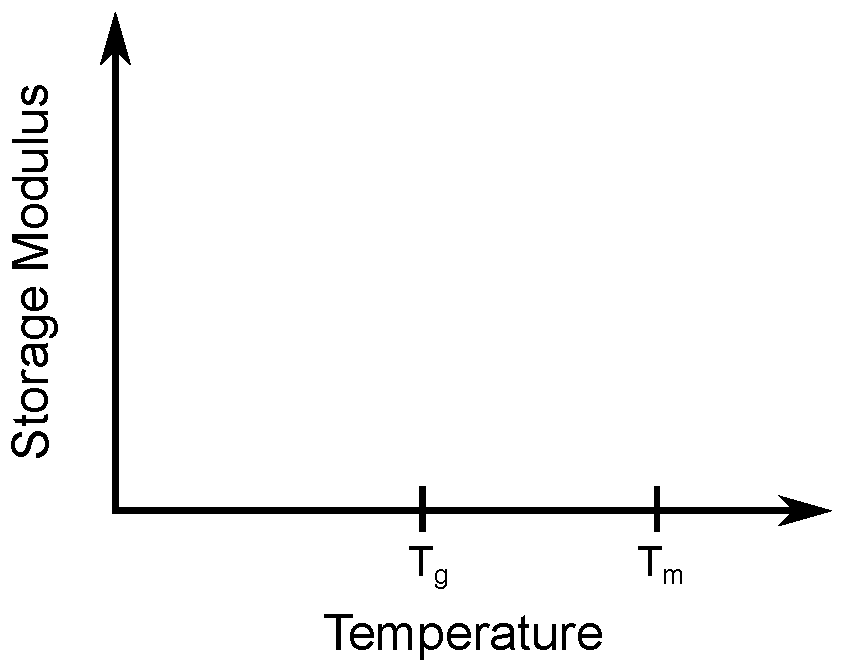
\includegraphics[width=0.5\textwidth]{\figpath/Model1_modulus_blank}}
		}\instructordisplay{
			\centerline{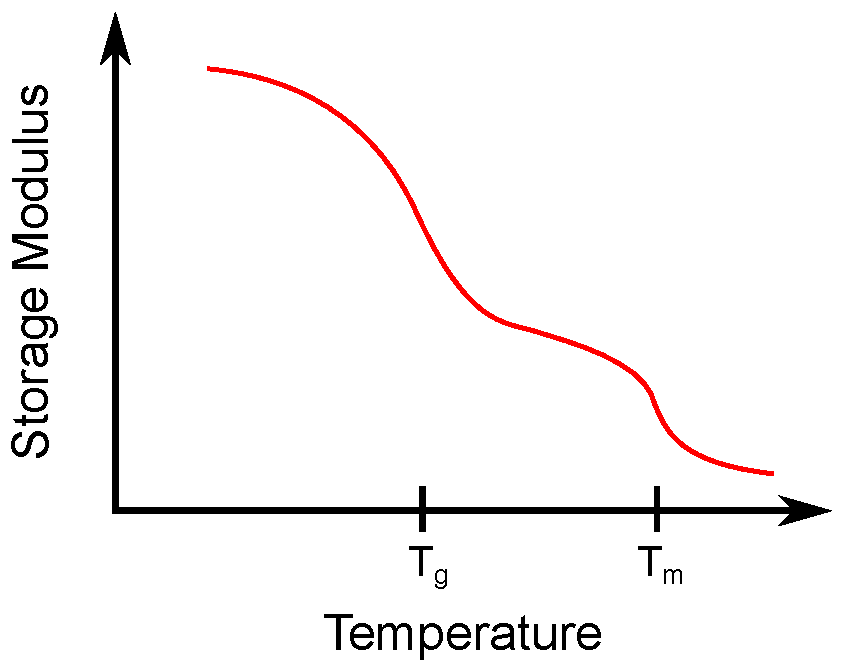
\includegraphics[width=0.5\textwidth]{\figpath/Model1_modulus_soln}}
		}\end{solution}
		
	
	\clearpage
	\question The modulus of a sample of polycarbonate, measured by DMA, is shown below:
	
		\vspace{6pt}
		\begin{solution}[2.5in]\studentdisplay{
			\centerline{
\includegraphics[width=0.35\textwidth]{\figpath/Model1_polycarbonateDMA}}
		}\instructordisplay{
			\centerline{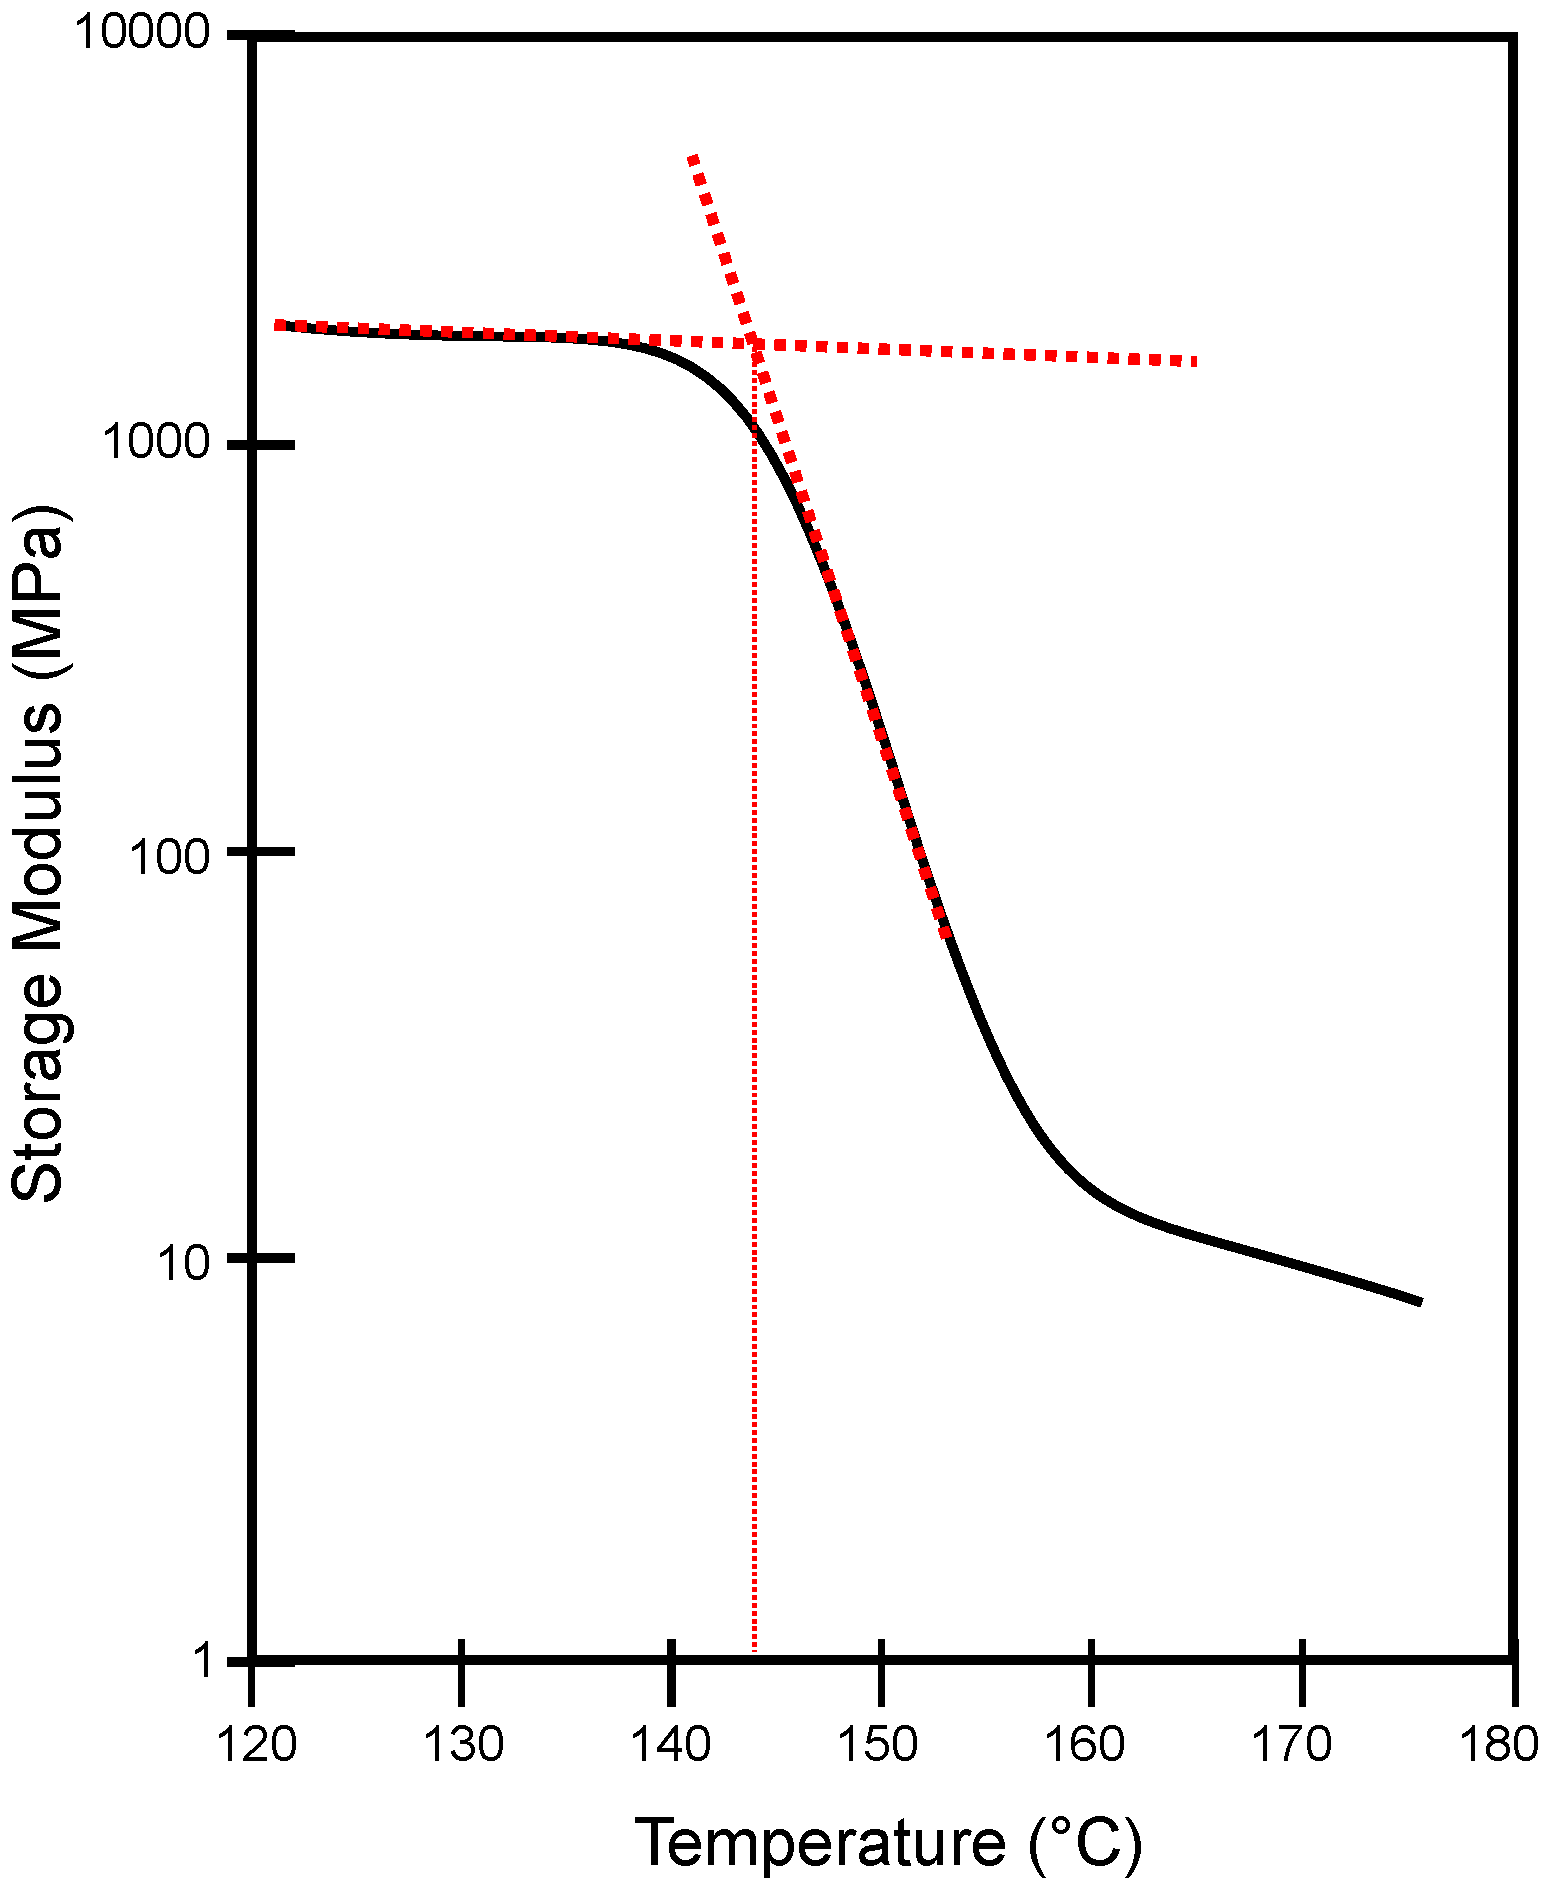
\includegraphics[width=0.35\textwidth]{\figpath/Model1_polycarbonateDMA-annotated}}
		}\end{solution}
		
		What value would your group report as the glass transition temperature of this material?  Briefly explain your reasoning in 1-2 complete sentences.
		
		\emph{Note: in this temperature range, polycarbonate only exhibits a $T_g$; no $T_m$ is observed.}
		
		\begin{solution}[1in]
			Any temperature between about 140 and 150 C would be a reasonable estimate.  The construction shown on the plot, above, is the tangent line construction used to find the onset $T_g$ from the modulus; this approach gives $T_g \approx 144$~C.
			
			Note that $T_g$ is often also determined in DMA experiments from the peak in the loss tangent, $\tan\delta = G''/G'$. While beyond the scope of this activity, this approach is conceptually useful because it identifies the temperature at which the timescale for segmental motion is one over the oscillation frequency at which the measurement is made - e.g. for measurements made at 1~rad/s, the peak in the loss tangent occurs at the temperature at which the timescale for segmental motion is approximately 1~s.
		\end{solution}
	
\end{ctqs}

%begin{infobox}
	
%	Often, it is easier to locate the glass transition by looking for either (i) a peak in the loss modulus, or (ii) a peak in the ratio of the storage and loss moduli (also referred to as $\tan\delta$).
	
%\end{infobox}

% would like to add a few CTQs getting at the idea that the peak in E'' occurs at the temperature at which the relaxation time is approx 1 s, but I think this requires more knowledge of the Maxwell Model than my students will realistically have

% could also turn into an exercise - maybe even get at the fact that you measure different Tg's with different deformation frequencies?

\begin{model}[Differential Scanning Calorimetry]
	
	Another common method for measuring $T_g$ and $T_m$ is \emph{differential scanning calorimetry} (DSC).  In a DSC experiment, the sample is heated at a constant rate, and the instrument measures the amount of heat (relative to a ``blank'' reference sample) that needs to be put in to maintain this constant rate of heating.
	
	For a sample with a constant heat capacity, a DSC experiment yields a flat line, as shown below:
	
		\centerline{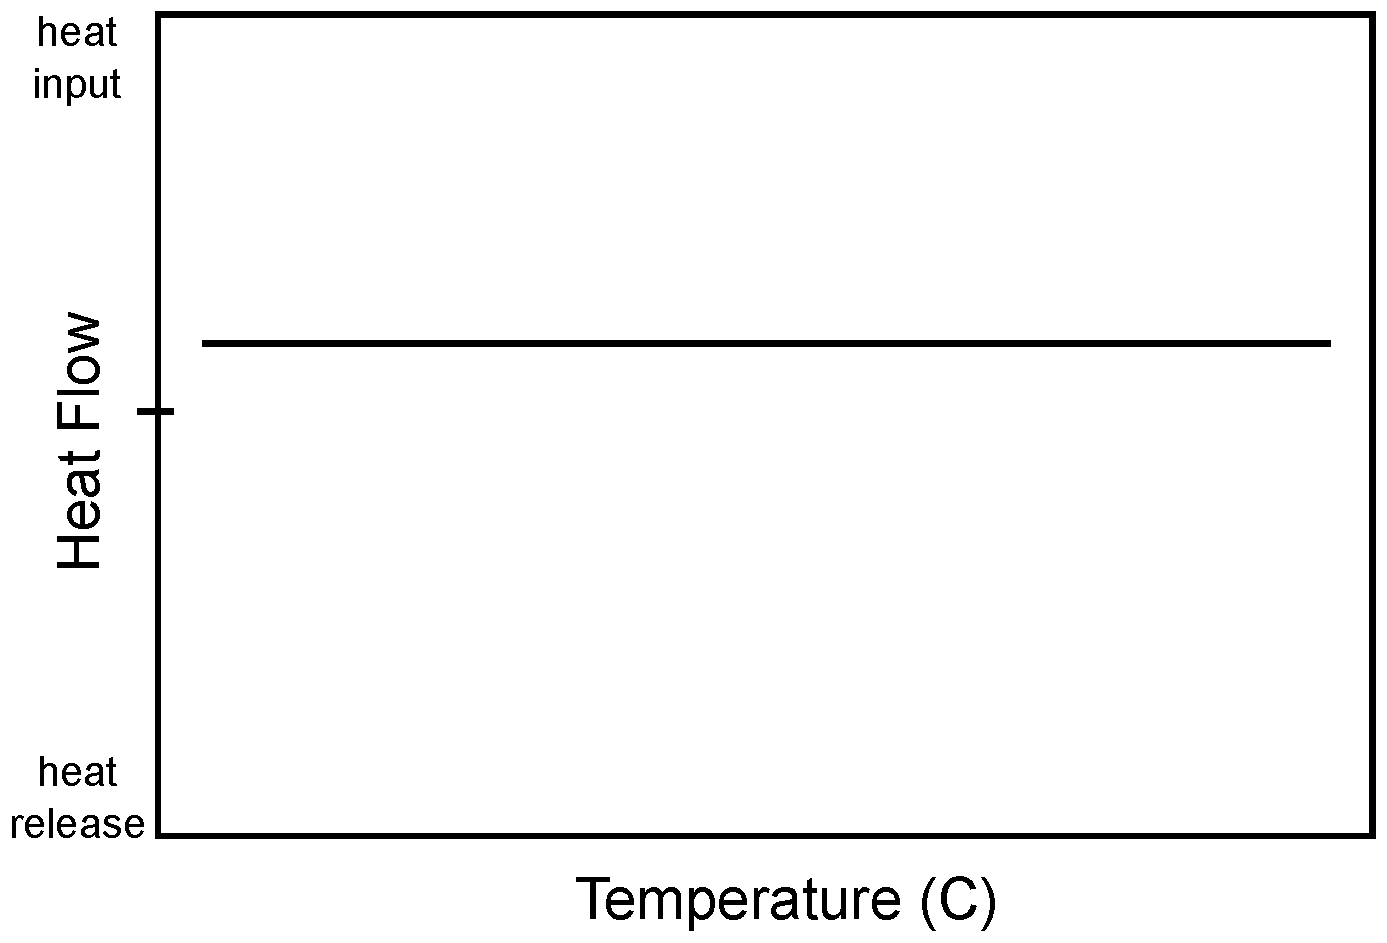
\includegraphics[width=0.5\textwidth]{\figpath/Model2_constCp}}
	
\end{model}

\begin{ctqs}

	\question Recall that the heat capacity of a material, $C_P$, is defined by
		\begin{equation*}
			C_p = \lim_{\Delta T\to 0} \frac{\Delta Q}{\Delta T}
		\end{equation*}
		where $\Delta Q$ is the amount of heat required to raise the temperature of the material by temperature $\Delta T$.
		
		Explain, in 1-2 complete sentences, why a material with constant $C_p$ gives a flat line in DSC.
		
			\begin{solution}[1in]
				If the heat capacity is constant, then each degree of temperature increase requires the same amount of heat to be transferred to the material.  The heat flow thus ends up being constant.
				%Note also that, for measurements made at constant temperature, $C_p = \left(\frac{\partial H}{\partial T}\right)_P$
			\end{solution}
		
	\question Suppose that a material's heat capacity increases (from $C_{p,1}$ to $C_{p,2}$) at some temperature $T_0$.  What shape would you expect the resulting DSC curve to have?  Sketch your group's answer on the axes below: \label{\labelbase:ctq:CPincrease}
	
		\vspace{6pt}
		\begin{solution}[2in]\studentdisplay{
			\centerline{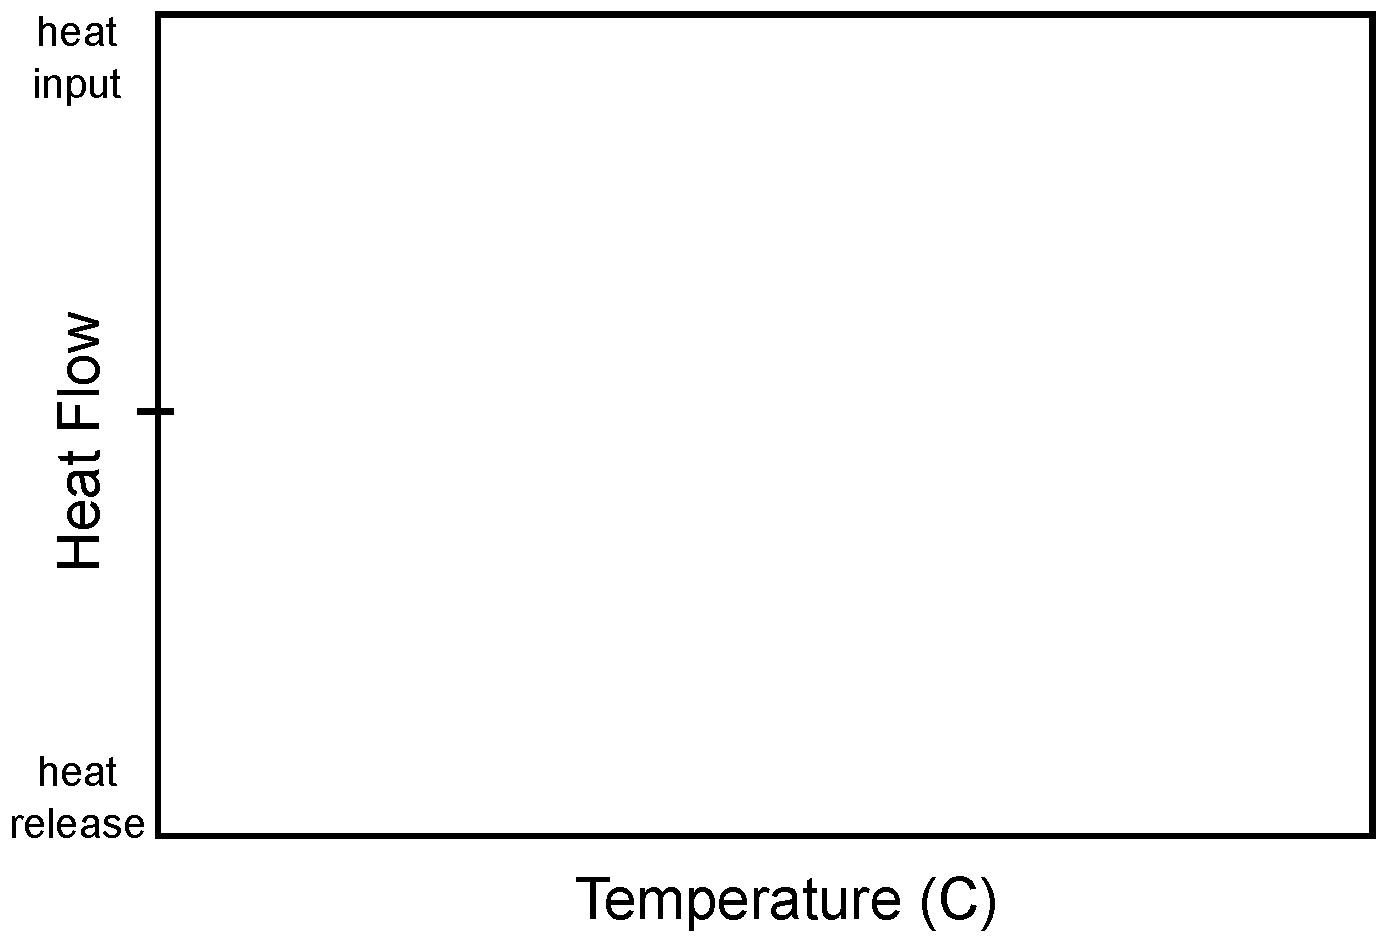
\includegraphics[width=0.45\textwidth]{\figpath/Model2_blankaxes}}
		}\instructordisplay{
			\centerline{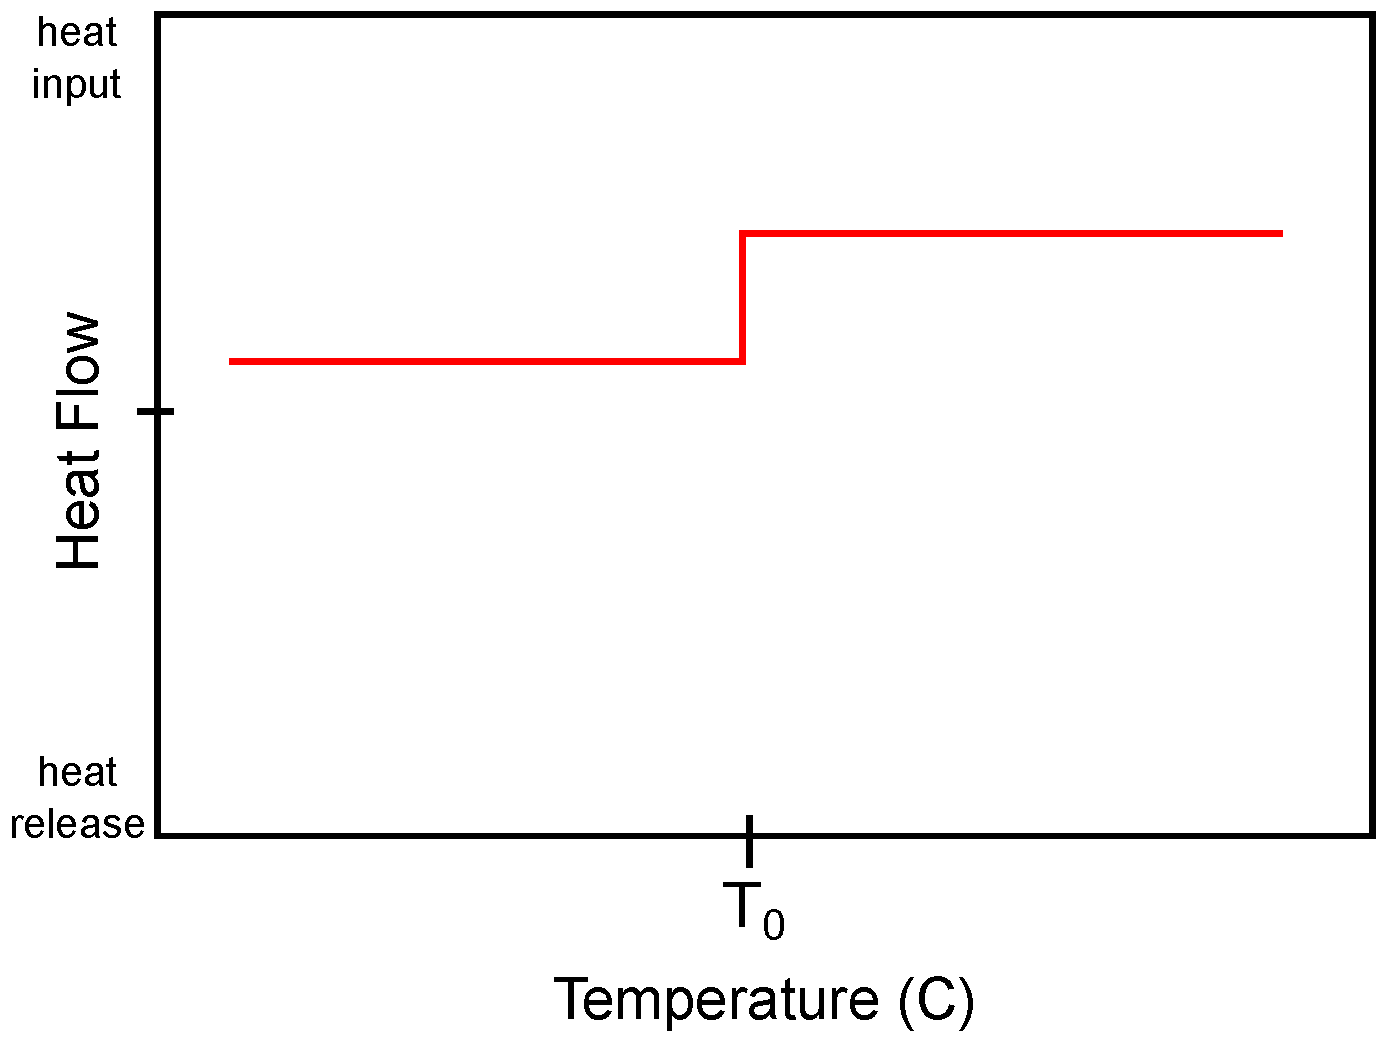
\includegraphics[width=0.45\textwidth]{\figpath/Model2_Tg_soln}}
		}\end{solution}
		
	\question Suppose that at temperature $T_0$, a significant amount of heat must be input to break apart some type of intermolecular interaction before the temperature of the sample can keep increasing.  What shape would you expect the resulting DSC curve to have?  Sketch your group's answer on the axes below.\label{\labelbase:ctq:delHtrans}
	
		\emph{For this question, you may assume that $C_p$ is the same before and after the transition.}
	
		\vspace{6pt}
		\begin{solution}[2in]\studentdisplay{
			\centerline{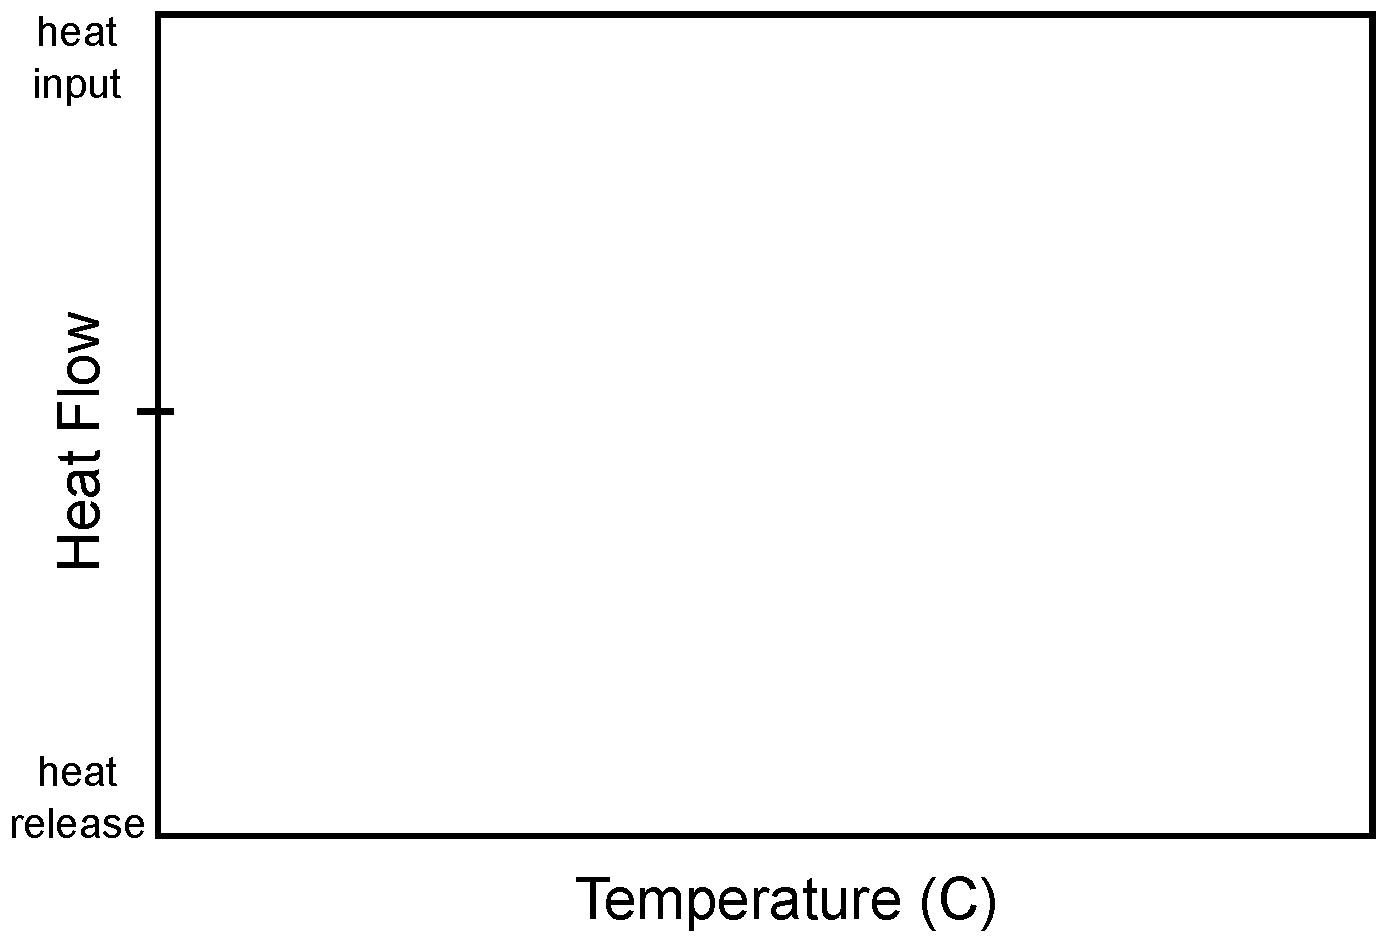
\includegraphics[width=0.45\textwidth]{\figpath/Model2_blankaxes}}
		}\instructordisplay{
			\centerline{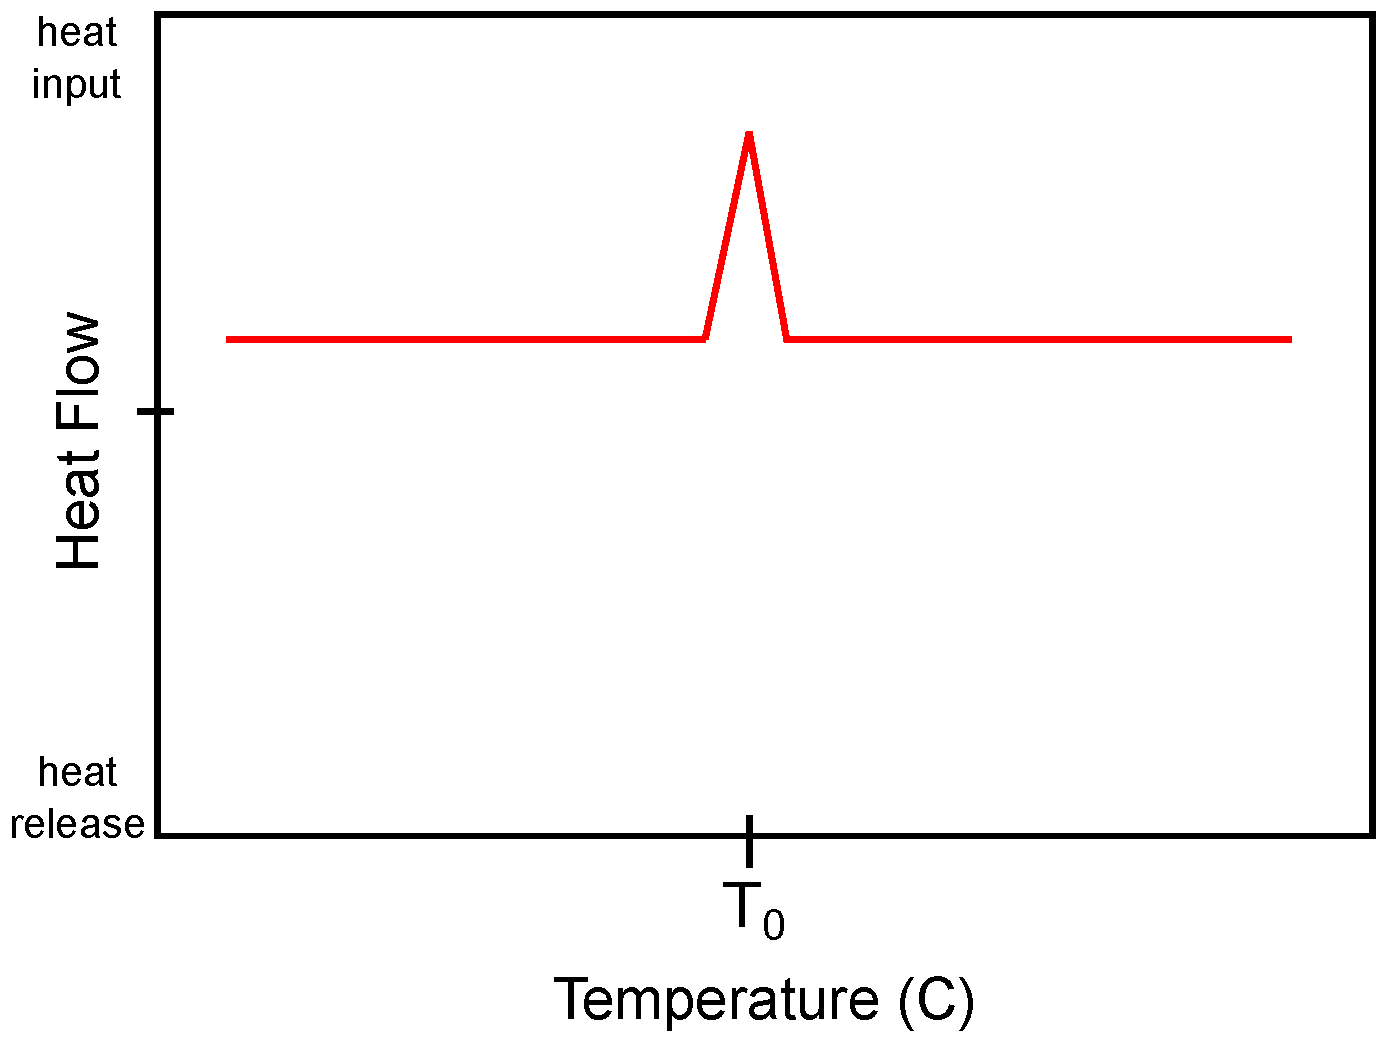
\includegraphics[width=0.45\textwidth]{\figpath/Model2_Tm_soln}}
		}\end{solution}
		
	\question Which of the two cases sketched above (CTQ \ref{\labelbase:ctq:CPincrease} or CTQ \ref{\labelbase:ctq:delHtrans}) do you expect to best describe the \emph{melting transition} of a crystalline polymer?  Briefly explain your group's reasoning in 1-2 complete sentences.
	
		\begin{solution}[2in]\studentdisplay{
		}\instructordisplay{
			The case sketched in CTQ \ref{\labelbase:ctq:delHtrans} best describes the melting transition of a crystalline polymer.  During the melting transition, heat must be supplied to break apart favorable interactions between the molecules.  This process occurs at a constant temperature (the melting temperature) and the temperature does not begin increasing again until the entire sample has melted.
			
			Note 1: If students are stuck on this, encourage them to think about what happens when ice melts.
			
			Note 2: here, we've made the simplifying assumption that $C_p$ is the same before and after the transition.  In practice, however, the heat capacity of the crystal and the heat capacity of the melt are not usually the same, so there will be a baseline offset before and after the melting peak resulting from this change in $C_p$.
		}\end{solution}
	
	\question Which of the two cases sketched above do you expect to best describe the \emph{glass transition} of a glassy polymer?  Briefly explain your group's reasoning in 1-2 complete sentences.
	
		\begin{solution}[2in]\studentdisplay{
		}\instructordisplay{
			The case sketched in CTQ \ref{\labelbase:ctq:CPincrease} best describes the glass transition of a glassy polymer. Because the glass transition temperature simply reflects a physical jamming of the molecules and does not arise from any specific \emph{interactions} between them, there are no interactions that need to be broken apart to push the material through its glass transition, and as a result, $T_g$ is not associated with the type of spike in the heat flow expected for the melting transition of a crystalline polymer as described above.  However, because the material has more degrees of freedom once it is ``un-jammed'', its heat capacity typically increases as it passes through its glass transition, resulting in the step function shown in CTQ \ref{\labelbase:ctq:CPincrease}.
		}\end{solution}
	
	\question Sketch the shape of the DSC curve you would expect to measure for a polymer that has \emph{both} a glass transition \emph{and} a melting transition on the axes below:
	
		\vspace{6pt}
		\begin{solution}[2.5in]\studentdisplay{
			\centerline{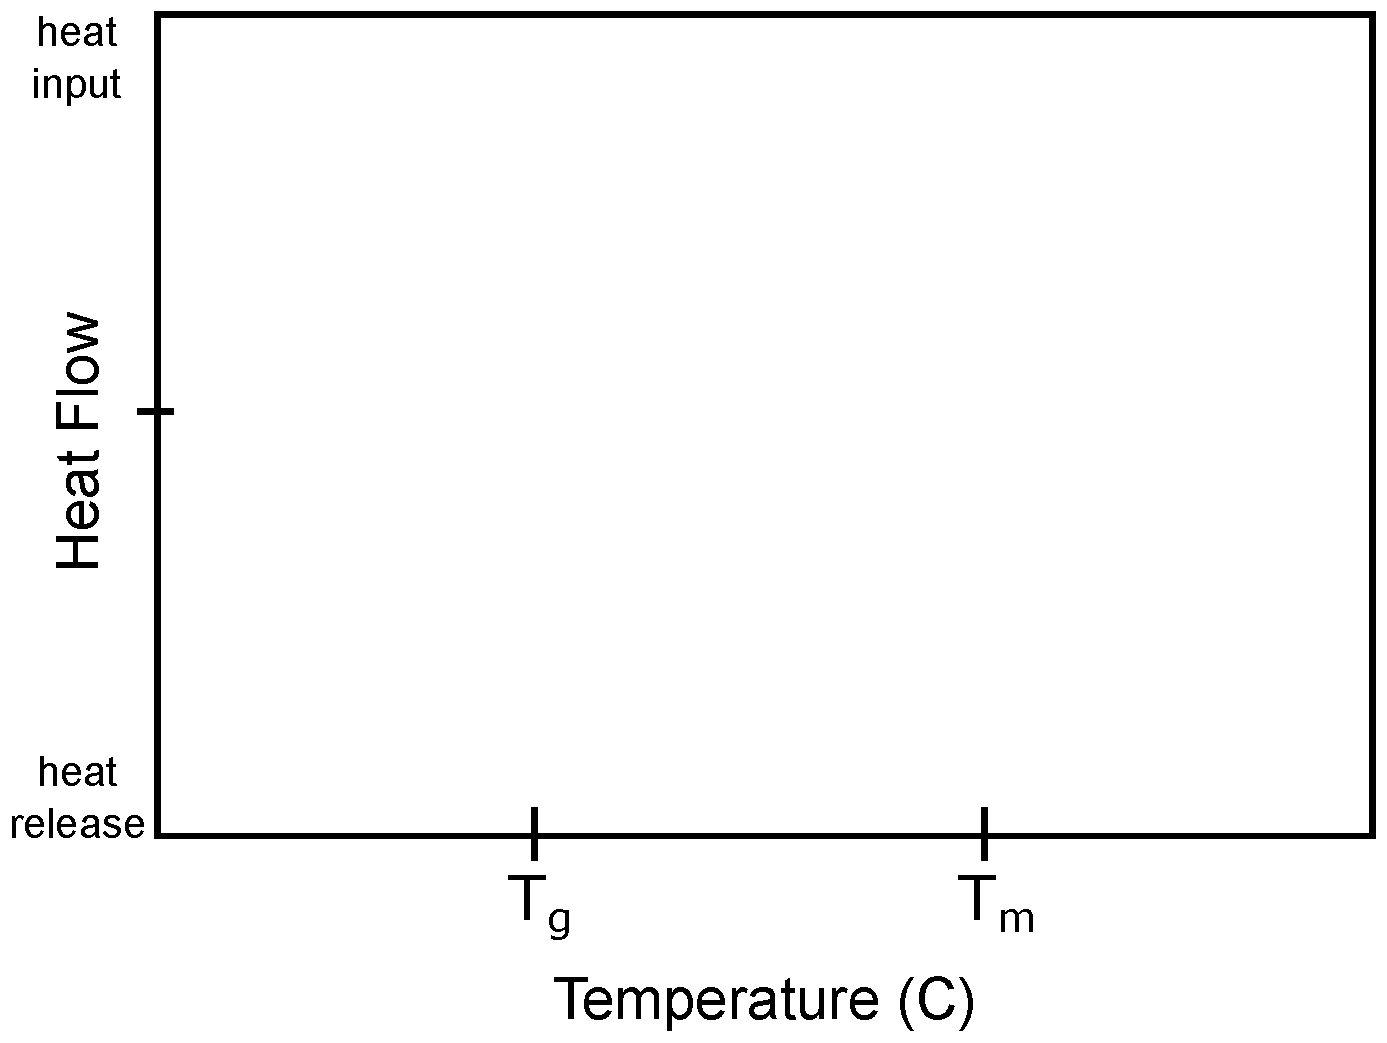
\includegraphics[width=0.55\textwidth]{\figpath/Model2_blankaxes_TgTm}}
		}\instructordisplay{
			\centerline{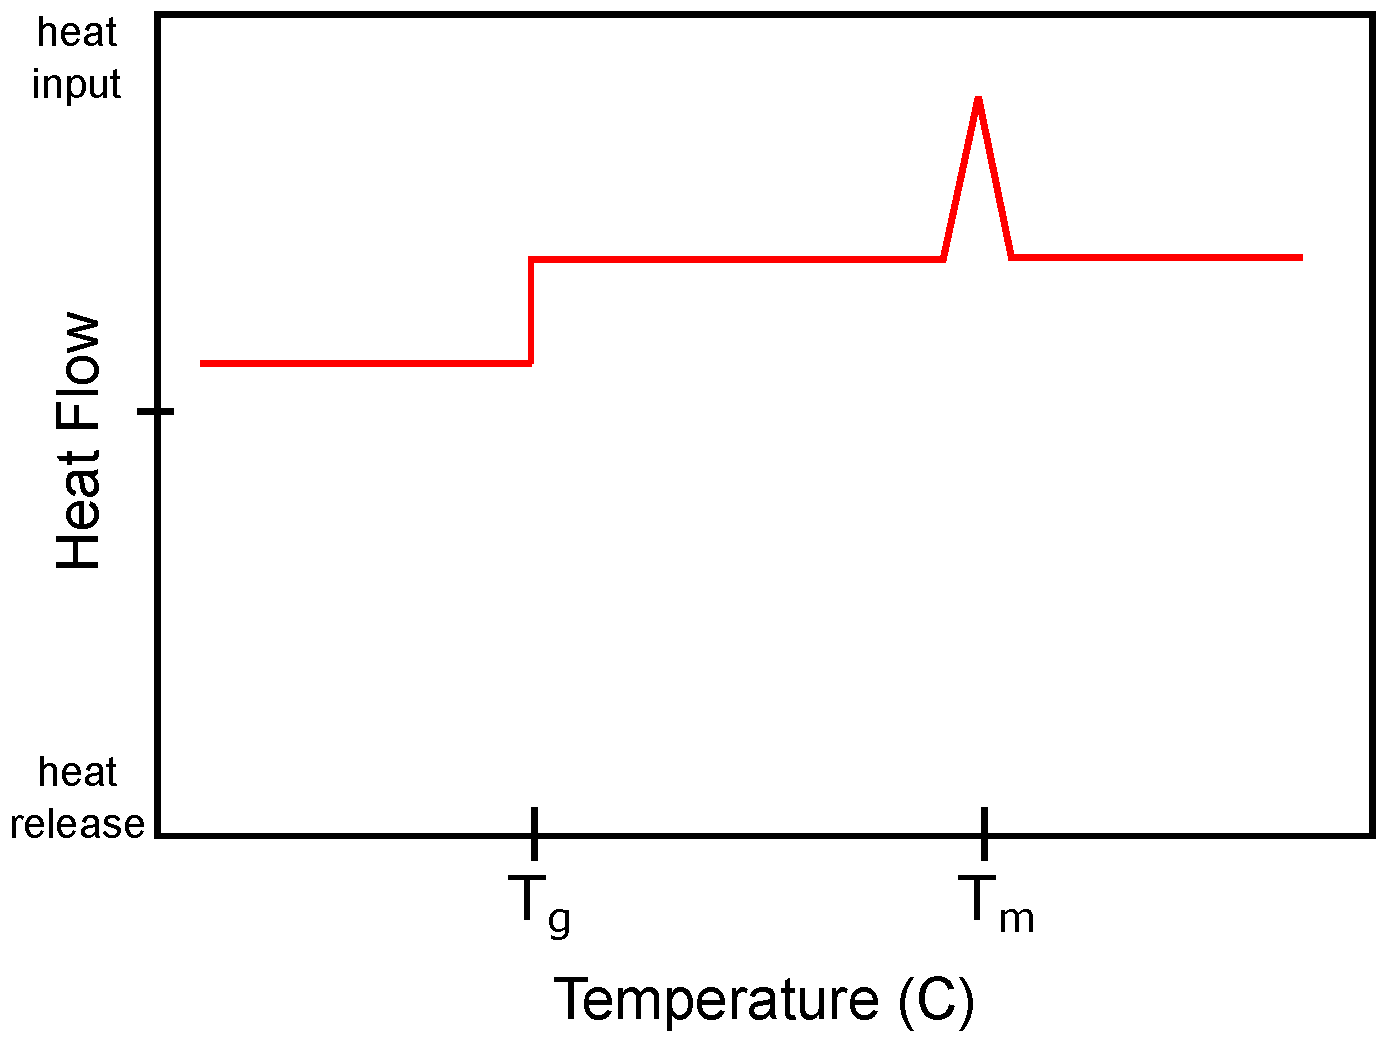
\includegraphics[width=0.55\textwidth]{\figpath/Model2_TgTm_soln}}
		}\end{solution}
	
	\clearpage
	\question A DSC trace measured for polyethyleneterephthalate (PET) is shown below:
	
		\vspace{6pt}
		\centerline{
\includegraphics[width=0.5\textwidth]{\figpath/Model2_PET}}
	
		\begin{enumerate}
			\item What is the glass transition temperature for this material?
			
				\begin{solution}[0.5in]
					Approx. 75-80~$^\circ$C
				\end{solution}
			
			\item What is the melting temperature for this material?
			
				\begin{solution}[0.5in]
					Approx. 250~$^\circ$C
				\end{solution}
			
			\item Are there any unexpected features in this curve? If so, what do the sign and shape of these feature(s) suggest about the process(es) they might represent?
			
				\begin{solution}[2in]
					Yes, there is an unexpected exothermic peak at about 160~$^\circ$C.  The sign of the peak (negative, corresponding to heat release) suggests that it arises from a process that \emph{forms} favorable interactions, and since it is essentially the same shape as the melting peak, we might guess that it reflects \emph{crystallization} of polymer chains.
					
					As it turns out, this peak is indeed a crystallization peak; when polymers are cooled they usually do not crystallize completely, and as the temperature is ramped up in the DSC experiment some of the chain segments may gain enough mobility to crystallize at an intermediate temperature between $T_g$ and $T_m$.
				\end{solution}
		\end{enumerate}
	
\end{ctqs}





%\begin{exercises}

%	\exercise A question about the loss tangent & timescale in DMA?
%
%	\exercise A question getting at heating rate in DSC?  And/or enthalpy overshoots?
%
%	\exercise A question getting at using the size of the $T_c$ peak to estimate the percent crystallinity of a material? (need to know enthalpy of fusion, so would need to make connection between heat flow and enthalpy (integral!) to get there.
	
%\end{exercises}


%\begin{problems}
%
%	\problem First exercise
%	\problem Second exercise
%	
%\end{problems}


	
\end{activity}